\section{Hamilton Reboots the Universe: When Motion Became a Coordinate System}

\subsection{Hamilton Reframes the Question: What Is Motion Made Of?}

As the 19\textsuperscript{th} century unfolded, the mathematical picture of nature was growing richer and more intricate. Newton had given the laws of motion; Lagrange had rewritten them as principles of least action; Laplace had described how fields curve in empty space; and Poisson had gone one step further, showing how matter itself bends these fields by sourcing them.

But in all of these approaches, the evolving state of a system was still treated as a sequence of positions — a path traced out in time or a field shaped across space.

Enter \textbf{William Rowan Hamilton}.

Hamilton saw that something even deeper connected these seemingly separate threads: a hidden geometry that unified motion, fields, and forces into one framework. His insight was not merely about predicting motion, but understanding its internal architecture — not just where things go, but how the very rules governing movement emerge from deeper symmetries.

If Newton gave us the laws,\\
and Lagrange gave us the principle,\\
and Laplace gave us the fields,\\
and Poisson gave us the sources,\\
then Hamilton gave us the \textbf{structure}.

He recast motion not simply as positions evolving through time, but as a smooth, continuous flow through a richer arena called \emph{phase space}, where position and momentum are treated as independent but equally fundamental coordinates. In this space, the full state of any system at any instant becomes a single point, and its evolution is a trajectory through this abstract landscape.

The question Hamilton posed was deceptively simple:

\begin{quote}
\textit{What happens when we separate position and motion into distinct coordinates — and treat them as equals?}
\end{quote}

\medskip

Where Poisson and Laplace had explored how fields curve under second derivatives, Hamilton recognized that for dynamical systems, the true flow arises from first derivatives — not of fields in space, but of an abstract scalar function called the \textbf{Hamiltonian}, typically representing total energy \( H = T + V \).

The Hamiltonian governs the system’s evolution through a pair of first-order relations:

\[
\frac{dq_i}{dt} = \frac{\partial H}{\partial p_i},
\qquad
\frac{dp_i}{dt} = -\frac{\partial H}{\partial q_i}.
\]

These are Hamilton’s equations: a compact, elegant reformulation where the system's entire behavior is determined by gradients of energy in phase space — just as Laplace and Poisson had described spatial gradients of potential fields.

\medskip

In this sense, Hamilton’s formalism unified all the Enlightenment approaches into one overarching structure:

\begin{itemize}
    \item \textbf{Lagrange} asked: which path extremizes action?
    \item \textbf{Laplace} asked: how do fields balance curvature?
    \item \textbf{Poisson} asked: how does matter create curvature?
    \item \textbf{Hamilton} asked: how does the entire system flow through state space, governed by energy gradients?
\end{itemize}

Each provided a different facet of the same grand vision: that nature’s complexity arises from simple, elegant principles — organizing motion, matter, and energy into a single logical structure.







\subsection{The Leap from Lagrange to Hamilton, in Hamilton’s Own Style}

Hamilton began by introducing the new variables
\[
p_i \;=\;\frac{dL}{d\dot q_i}
\]
and defining a function \(H\) of the coordinates \(q_i\), the momenta \(p_i\), and time \(t\) by
\[
H \;=\;\sum_{i=1}^n p_i\,\dot q_i \;-\; L.
\]
He then considered the total change of \(H\) under small variations of its arguments:
\[
dH
\;=\;
A_1\,dq_1 + \cdots + A_n\,dq_n
\;+\;
B_1\,dp_1 + \cdots + B_n\,dp_n
\;+\;
C\,dt,
\]
where each coefficient \(A_i\) is the change in \(H\) when \(q_i\) alone is varied, \(B_i\) the change when \(p_i\) alone is varied, and \(C\) the change when \(t\) alone is varied.

If \(H\) does not depend explicitly on \(t\), then along a true motion \(dH=0\).  Since the increments \(dq_i\), \(dp_i\), and \(dt\) are independent, Hamilton deduced for each \(i\):
\[
\frac{dq_i}{dt} = B_i,
\qquad
\frac{dp_i}{dt} = -\,A_i,
\qquad
C = 0.
\]
These equations—expressing the rates of change of position and momentum directly in terms of the coefficients \(A_i\) and \(B_i\)—are exactly Hamilton’s equations, written in the language and notation of his own time, without invoking modern partial derivatives. 



\subsection{Conjugate Momentum}

Every generalized coordinate \(q_i\) in Lagrange’s formulation comes equipped with its own \emph{conjugate momentum}, defined by
\[
p_i \;=\;\frac{dL}{d\dot q_i}.
\]
Physically, \(p_i\) measures how the Lagrangian—and hence the action—changes when we vary the velocity \(\dot q_i\) alone, holding all other coordinates and velocities fixed.

\medskip

\noindent\textbf{Examples of Conjugate Momentum}
\begin{itemize}
  \item \emph{Cartesian coordinate \(x\):} \(\;p_x = \tfrac{d}{d\dot x}\bigl(\tfrac12\,m\,\dot x^2 - V\bigr) = m\,\dot x,\) the familiar linear momentum.
  \item \emph{Angular coordinate \(\theta\):} \(\;p_\theta = \tfrac{d}{d\dot\theta}\bigl(\tfrac12\,m\,r^2\dot\theta^2 - V\bigr) = m\,r^2\,\dot\theta,\) the angular momentum about the chosen origin.
  \item \emph{Arc‐length \(s\) along a curve:} \(\;p_s = m\,\dot s,\) the momentum along the path.
\end{itemize}

\bigskip
Because \(p_i\) arises directly from the Lagrangian, it transforms correctly under changes of generalized coordinates and encodes any constraints or geometry built into \(L\).  Moreover, if the coordinate \(q_j\) does not appear explicitly in \(L\), then by Lagrange’s recipe
\[
\frac{d}{dt}\Bigl(p_j\Bigr) \;=\; 0,
\]
so the conjugate momentum \(p_j\) is conserved.  This is the deep connection between symmetries (cyclic coordinates) and conservation laws, and it underlies much of modern analytical mechanics.  

\begin{figure}[H]
    \centering
    \begin{tikzpicture}[>=stealth,scale=1]
      % Axes
      \draw[->] (-0.2,0) -- (3,0) node[right] {$\dot q$};
      \draw[->] (0,-0.2) -- (0,3) node[above] {$L$};
    
      % Parabola L = ½ m dot{q}^2 (m=1), now light dashed
      \draw[blue!50!white,dashed,domain=0:2.5,samples=100]
        plot (\x,{0.5*\x*\x});
    
      % Sample velocity dot q0
      \def\dq{1.5}
      \coordinate (P) at (\dq,{0.5*\dq*\dq});
      \filldraw[red] (P) circle (2pt);
    
      % Tangent line at P: slope = dq0
      \draw[red,dashed,domain=0:2.8]
        plot (\x,{0.5*\dq*\dq + \dq*(\x-\dq)});
    
      % Conjugate momentum arrow, made bolder
      \draw[->,green!60!black,very thick,line cap=round]
        (P) -- ++(0.5,0.5*\dq) coordinate (M);
      
      % Legend background
      \node[draw, fill=white, inner sep=5pt] at (-2.5,2.5) {
        \begin{tikzpicture}[>=stealth,scale=1, every node/.style={font=\footnotesize}]
          % Parabola legend
          \draw[blue!50!white,dashed] (0,0) -- (0.5,0) node[right]{\(L(\dot q)\)}; 
          % Tangent legend
          \draw[red,dashed] (0,-0.3) -- (0.5,-0.3) node[right]{tangent line}; 
          % Momentum arrow legend, bolder
          \draw[green!60!black,very thick,->] (0,-0.6) -- (0.5,-0.6) node[right]{\(p = \tfrac{dL}{d\dot q}\)};
        \end{tikzpicture}
      };
    
      % Annotations
      \node[above right] at (P) {$(\dot q_0,\,L_0)$};
      \node[right] at (M) {\(\displaystyle p = m\,\dot q_0\)};
    
    \end{tikzpicture}
    \caption{%
    Plot of \(L(\dot q)=\tfrac12m\dot q^2 - V\) (here \(m=1\), \(V=0\)) versus \(\dot q\).
    The light dashed blue curve is the action, and the bold green arrow shows the conjugate‐momentum slope.}
\end{figure}

    







\subsection{Phase Space: Motion as Geometry}

In Hamilton’s view, a system’s state at any instant is completely specified by the pair \((q_i,p_i)\).  Thus, instead of following a point in “configuration space” (where only the positions \(q_i\) vary), we follow a point in “phase space,” a two‐coordinate plane for each degree of freedom:

\begin{itemize}
  \item In configuration space, the path \(q(t)\) shows “where” the system is.
  \item In phase space, the path \(\bigl(q(t),p(t)\bigr)\) shows both “where” and “how fast” (via \(p\)) the system moves.
\end{itemize}

Qualitatively, this has several striking consequences:

\begin{enumerate}
  \item {\bf Energy contours become curves.}  For a conservative system of fixed total energy \(E\), the motion in phase space lies on a single closed curve (an “energy contour”).  
  \item {\bf Flow without crossings.}  Two trajectories never intersect, since from each phase‐space point the future (and past) are uniquely determined.
  \item {\bf Geometric insight.}  Simple motions (e.g.\ the harmonic oscillator) appear as ellipses, while more complex dynamics trace out more intricate loops or even fill regions densely.
\end{enumerate}

\medskip
\noindent\textbf{Example: Simple Harmonic Oscillator.}  
A mass on a spring of stiffness \(k\) satisfies \(p=m\,\dot q\), and its energy 
\[
E \;=\; \tfrac12\,m\,\dot q^2 \;+\;\tfrac12\,k\,q^2
\]
becomes the constant
\[
\tfrac{p^2}{2m} + \tfrac12\,k\,q^2 = E.
\]
In the \((q,p)\) plane this is the ellipse
\[
\frac{q^2}{( \sqrt{2E/k} )^2} + \frac{p^2}{( \sqrt{2mE} )^2} = 1,
\]
traced continuously as time evolves.

\begin{figure}[H]
\centering
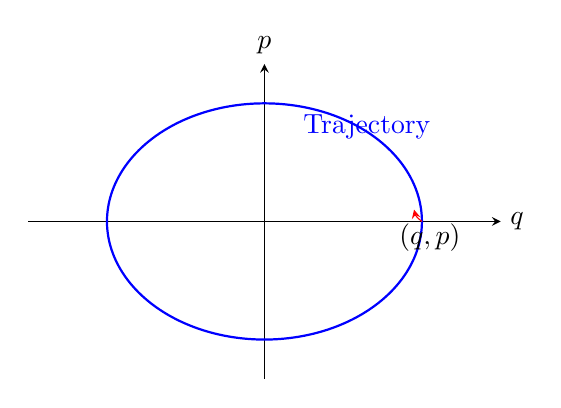
\begin{tikzpicture}[>=stealth, scale=1]
  % Axes
  \draw[->] (-3,0) -- (3,0) node[right] {$q$};
  \draw[->] (0,-2) -- (0,2) node[above] {$p$};
  % Ellipse: a = 2, b = 1.5
  \draw[thick,blue,domain=0:360,smooth,samples=200]
    plot ({2*cos(\x)}, {1.5*sin(\x)});
  % Direction arrow
  \draw[red,->] (2,0) to[bend left=20] (1.9,0.15);
  % Labels
  \node[blue] at (1.3,1.2) {Trajectory};
  \node at (2.1, -0.2) {$(q,p)$};
\end{tikzpicture}
\caption{Phase‐space ellipse for a simple harmonic oscillator of energy \(E\).}
\end{figure}

This depiction shows how the oscillator’s state flows around the ellipse without ever crossing itself, giving a complete geometric picture of its motion in the plane of position and momentum.  











\subsection{Symplectic Geometry: Mechanics Becomes Geometry}

In the Hamiltonian picture, each state of the system is a point \((q_i,p_i)\) in phase space, and the evolution of the system traces out a curve in this higher-dimensional arena.  Unlike Lagrange’s emphasis on extremizing an action, Hamilton saw that these curves are the integral lines of a vector field—one that preserves a fundamental “area” element in phase space.

Concretely, if we pair up each coordinate \(q_i\) with its conjugate momentum \(p_i\), we obtain the 2-form
\[
\omega \;=\;\sum_i dq_i\wedge dp_i,
\]
which assigns an oriented “signed area” to each infinitesimal parallelogram in phase space.  Hamilton’s equations then generate a flow that carries each such parallelogram into another of \emph{exactly} the same area.  No squeezing, no stretching—just pristine volume preservation.

This invariance of \(\omega\) under the flow is the geometric heart of \textbf{Liouville’s Theorem}: the phase-space density of an ensemble of systems remains constant along trajectories.  What Lagrange gave us as an algebra of variation, Hamilton elevated to a \emph{geometry of flow}, where the very shape and volume of regions in phase space are inviolate.

\begin{figure}[H]
\centering
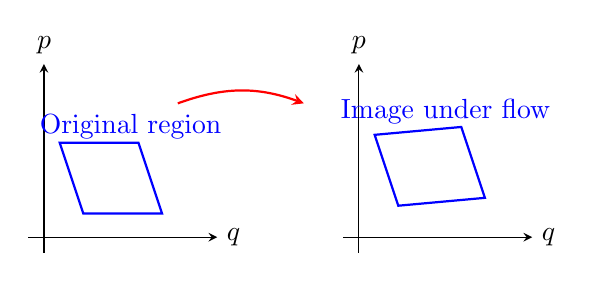
\begin{tikzpicture}[>=stealth, scale=1]
  % Left axes and original parallelogram
  \draw[->] (-0.2,0) -- (2.2,0) node[right] {$q$};
  \draw[->] (0,-0.2) -- (0,2.2) node[above] {$p$};
  \draw[thick, blue] (0.5,0.3) -- (1.5,0.3) -- (1.2,1.2) -- (0.2,1.2) -- cycle;
  \node[blue] at (1.1,1.4) {Original region};

  % Flow arrow
  \draw[->, red, thick] (1.7,1.7) to[bend left=20] (3.3,1.7);

  % Right axes and image parallelogram
  \begin{scope}[xshift=4cm]
    \draw[->] (-0.2,0) -- (2.2,0) node[right] {$q$};
    \draw[->] (0,-0.2) -- (0,2.2) node[above] {$p$};
    \draw[thick, blue] (0.5,0.4) -- (1.6,0.5) -- (1.3,1.4) -- (0.2,1.3) -- cycle;
    \node[blue] at (1.1,1.6) {Image under flow};
  \end{scope}
\end{tikzpicture}
\caption{A small region in the \((q,p)\) plane is carried by the Hamiltonian flow into another region of identical signed area, illustrating preservation of the symplectic form \(\omega=dq\wedge dp\).}
\end{figure}

\begin{quote}
    \textit{Lagrange optimized paths; Hamilton mapped out the unchanging geometry of motion.}
\end{quote}






\subsection{Energy Trajectories in Phase Space}

Before defining energy trajectories, we first introduce the notion of a \emph{level set}.  Given any function \(F\) on a plane—say \(F(x,y)\)—the level set at value \(c\) is the collection of all points \((x,y)\) for which

\[
F(x,y) = c.
\]

Geometrically, this is a curve (or collection of curves) along which the function remains constant.

In a Hamiltonian system, the total energy

\[
H(q,p) \;=\; T(p) + V(q)
\]

plays the role of \(F\).  Its level set

\[
H(q,p) = E
\]

is therefore the \emph{energy trajectory} in the \((q,p)\) plane: the curve along which the system moves because its energy \(E\) is conserved.

\textbf{Example: Simple Harmonic Oscillator.}  

For

\[
T = \frac{p^2}{2m}
\quad\text{and}\quad
V = \tfrac12\,k\,q^2,
\]

the equation

\[
\frac{p^2}{2m} + \frac12\,k\,q^2 = E
\]

is a level set of \(H\)—an ellipse in phase space.  As the oscillator evolves, its state \((q(t),p(t))\) traces this ellipse without ever leaving it.

\begin{figure}[H]
\centering
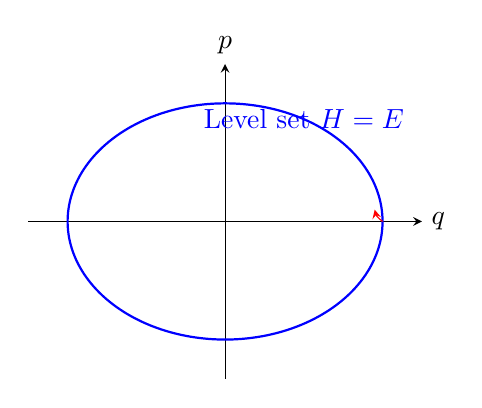
\begin{tikzpicture}[>=stealth, scale=1]
  % Axes
  \draw[->] (-2.5,0) -- (2.5,0) node[right] {$q$};
  \draw[->] (0,-2) -- (0,2) node[above] {$p$};
  % Energy‐trajectory ellipse
  \draw[thick,blue,domain=0:360,smooth,samples=200]
    plot ({2*cos(\x)}, {1.5*sin(\x)});
  % Direction arrow
  \draw[red,->] (2,0) to[bend left=20] (1.9,0.15);
  % Labels
  \node[blue] at (1,1.3) {Level set \(H=E\)};
\end{tikzpicture}
\caption{The level set \(H(q,p)=E\) in the \((q,p)\) plane is the energy trajectory of the simple harmonic oscillator, here an ellipse defined by \(\tfrac{p^2}{2m} + \tfrac12\,k\,q^2 = E\).}
\end{figure}

Because the Hamiltonian flow preserves the symplectic form \(\omega\), the system’s state moves along this level‐set curve without crossing it or changing the enclosed area, providing a vivid geometric picture of energy conservation.  







\subsection{Kepler’s Second Law in Angular Phase Space}

Because the angle \(\theta\) does not appear explicitly in the Hamiltonian, its conjugate momentum
\[
p_\theta \;=\; m\,r^2\,\dot\theta
\]
remains constant.  We may therefore plot the motion in the \((\theta,p_\theta)\) plane:

\begin{itemize}
  \item Horizontal axis: \(\theta\).
  \item Vertical axis: \(p_\theta\).
\end{itemize}

The trajectory is simply the horizontal line \(p_\theta=\text{const}\).  The phase‐space area under that line between two angles \(\theta_1\) and \(\theta_2\) is
\[
\int_{\theta_1}^{\theta_2} p_\theta\,d\theta
\;=\;
p_\theta\,(\theta_2-\theta_1).
\]
Symplectic area conservation then tells us that this “phase‐space area” is proportional to the physical area \(\Delta A\) swept in the real orbit:
\[
\Delta A \;=\;\tfrac{1}{2m}\,p_\theta\,\Delta\theta.
\]
Hence equal increments \(\Delta\theta\) in equal times produce equal \(\Delta A\), exactly Kepler’s Second Law.

\begin{figure}[H]
\centering
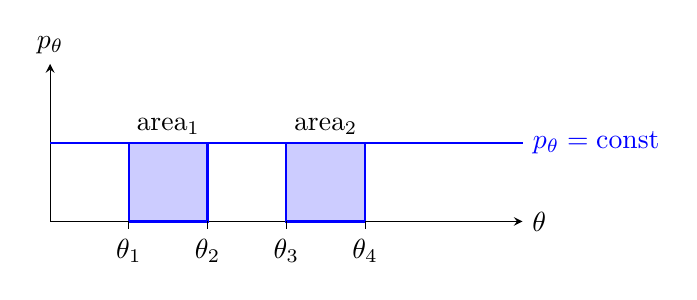
\begin{tikzpicture}[>=stealth, scale=1]
  % Axes
  \draw[->] (0,0) -- (6,0) node[right] {$\theta$};
  \draw[->] (0,0) -- (0,2) node[above] {$p_\theta$};
  % Constant momentum line
  \draw[thick,blue] (0,1) -- (6,1) node[right] {$p_\theta=\mathrm{const}$};
  % Shaded equal-area rectangles
  \fill[blue!20] (1,0) rectangle (2,1);
  \fill[blue!20] (3,0) rectangle (4,1);
  \draw[blue,thick] (1,0) rectangle (2,1) (3,0) rectangle (4,1);
  % Angle ticks and labels
  \foreach \x/\lab in {1/\theta_1,2/\theta_2,3/\theta_3,4/\theta_4} {
    \draw (\x,0) -- (\x,-0.1) node[below] {\(\lab\)};
  }
  % Area labels
  \node at (1.5,1.2) {area$_1$};
  \node at (3.5,1.2) {area$_2$};
\end{tikzpicture}
\caption{In the \((\theta,p_\theta)\) plane, equal angular intervals \(\Delta\theta\) under the line \(p_\theta=\mathrm{const}\) sweep out equal phase‐space areas \(p_\theta\,\Delta\theta\), corresponding to equal physical areas in the orbit.}
\end{figure}

\begin{figure}[H]
    \centering
    % Define the sample angles locally
    \def\thA{30}
    \def\thB{80}
    
    % 1) Cartesian view
    \subcaptionbox{Physical orbit in the $(x,y)$ plane\label{fig:kepler-cartesian}}{%
      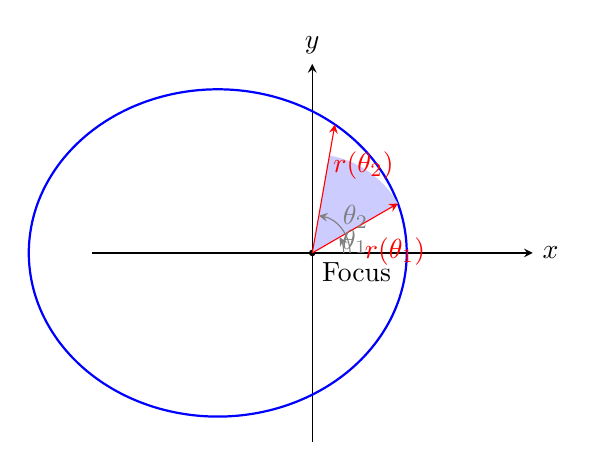
\begin{tikzpicture}[>=stealth,scale=0.8]
        % Axes
        \draw[->] (-3.5,0) -- (3.5,0) node[right] {$x$};
        \draw[->] (0,-3) -- (0,3) node[above] {$y$};
        % Ellipse (a=3, e=0.5)
        \draw[thick,blue,domain=0:360,smooth,samples=200]
          plot ({(2.25/(1+0.5*cos(\x)))*cos(\x)},
               {(2.25/(1+0.5*cos(\x)))*sin(\x)});
        % Focus
        \fill (0,0) circle (1.5pt) node[below right] {Focus};
        % Compute radii
        \pgfmathsetmacro\rA{2.25/(1+0.5*cos(\thA))}
        \pgfmathsetmacro\rB{2.25/(1+0.5*cos(\thB))}
        % Points at θ₁ and θ₂
        \coordinate (A) at ({\rA*cos(\thA)},{\rA*sin(\thA)});
        \coordinate (B) at ({\rB*cos(\thB)},{\rB*sin(\thB)});
        % Shaded wedge
        \fill[blue!20] (0,0) -- (A) arc[start angle=\thA,end angle=\thB,radius=\rA] -- cycle;
        % Radius vectors
        \draw[red,->] (0,0) -- (A) node[midway,below right] {$r(\theta_1)$};
        \draw[red,->] (0,0) -- (B) node[midway,above right] {$r(\theta_2)$};
        % Angle arcs
        \draw[gray,->] (0.5,0) arc[start angle=0,end angle=\thA,radius=0.5];
        \node[gray] at ({0.7*cos(\thA/2)},{0.7*sin(\thA/2)}) {$\theta_1$};
        \draw[gray,->] (0.6,0) arc[start angle=0,end angle=\thB,radius=0.6];
        \node[gray] at ({0.9*cos(\thB/2)},{0.9*sin(\thB/2)}) {$\theta_2$};
      \end{tikzpicture}
    }
    
    \vspace{1em}
    
    % 2) Phase‐space view (compressed horizontally)
    \subcaptionbox{Angular momentum phase space\label{fig:kepler-phase}}{%
      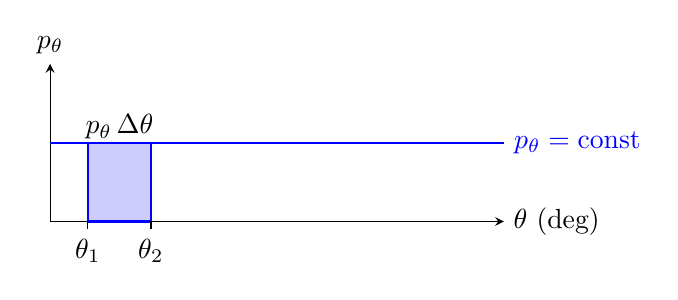
\begin{tikzpicture}[>=stealth,xscale=0.016,yscale=1]
        % Axes
        \draw[->] (0,0) -- (360,0) node[right] {$\theta$ (deg)};
        \draw[->] (0,0) -- (0,2)   node[above] {$p_\theta$};
        % Constant momentum line
        \draw[thick,blue] (0,1) -- (360,1) node[right] {$p_\theta=\mathrm{const}$};
        % Shade same angular wedge
        \fill[blue!20] (\thA,0) rectangle (\thB,1);
        \draw[blue,thick] (\thA,0) rectangle (\thB,1);
        % Tick labels
        \draw (\thA,0) -- ++(0,-0.1) node[below] {$\theta_1$};
        \draw (\thB,0) -- ++(0,-0.1) node[below] {$\theta_2$};
        % Area label
        \node at ({(\thA+\thB)/2},1.2) {$p_\theta\,\Delta\theta$};
      \end{tikzpicture}
    }
    
    \caption{%
    Comparison of Kepler’s Second Law in physical and phase‐space views.
    (\subref{fig:kepler-cartesian}) The elliptical orbit in the $(x,y)$ plane, with equal angular wedge between $\theta_1$ and $\theta_2$ shading equal physical areas.
    (\subref{fig:kepler-phase}) The corresponding phase‐space plot $(\theta,p_\theta)$ shows the same angular interval shading equal phase‐space area $p_\theta\,\Delta\theta$.}
\end{figure}
    